\documentclass[sigconf]{acmart}

\usepackage{booktabs} % For formal tables
\usepackage{amsmath}
\usepackage{bm}
\usepackage{float}
\usepackage{amsfonts}

\acmPrice{15.00}

% The next six lines come directly from the completed rights form.
% You MUST replace them with the lines specific to your accepted work.
\copyrightyear{2018}
\acmYear{2018}
\setcopyright{rightsretained}
\acmConference{Interactive 3D Graphics and Games}{2019}{Montreal}
\acmDOI{10.1145/8888888.7777777}
\acmISBN{978-1-4503-1234-5/17/07}

% Use the "authoryear" citation style, and make sure citations are in [square brackets].
\citestyle{acmauthoryear}
\setcitestyle{square}

% A useful command for controlling the number of authors per row.
% The default value of "authorsperrow" is 2.
\settopmatter{authorsperrow=4}

% end of preamble.
% --------------------------------------------------------------------------
\begin{document}

% Title. 
% If your title is long, consider \title[short title]{full title} - "short title" will be used for running heads.
\title{Deep Precomputed Radiance Transfer for Deforming Objects}

% Authors.
\author{Yue Li}
\affiliation{%
  \institution{University of Pensylvania??}}
\email{yueli.cg@gmail.com}

\author{Pablo Wiedemann}
\affiliation{%
  \institution{Edinburgh Napier University}}
\email{p.wiedemann@napier.ac.uk}

\author{Kenny Mitchell}
\affiliation{%
  \institution{Edinburgh Napier University}}
\email{k.mitchell2@napier.ac.uk}


% This command defines the author string for running heads.
\renewcommand{\shortauthors}{Li, Wiedemann,Mitchell}

% ----- ABSTRACT -----------------
\begin{abstract}
   Traditional Precomputed Radiance Transfer methods  require a lot of memory to save the precomputed data for real time rendering. For an animation sequence such data would be gigantic. We proposed a deep learning precomputed radiance transfer framework (DPRT) for deforming object, saving only the weights of the network, which lowers the memory cost in orders of magnitudes. Object is first parameterized via harmonic mapping and reconstructed to form geometry and normal image as the inputs of a carefully designed fully convolutional network. 
%-------------------------------------------------------------------------
%  ACM CCS 1998
%  (see http://www.acm.org/about/class/1998)
% \begin{classification} % according to http:http://www.acm.org/about/class/1998
% \CCScat{Computer Graphics}{I.3.3}{Picture/Image Generation}{Line and curve generation}
% \end{classification}
%-------------------------------------------------------------------------
%  ACM CCS 2012
   (see http://www.acm.org/about/class/class/2012)
%The tool at \url{http://dl.acm.org/ccs.cfm} can be used to generate
% CCS codes.
%Example:
\begin{CCSXML}
<ccs2012>
<concept>
<concept_id>10010147.10010371.10010352.10010381</concept_id>
<concept_desc>Computing methodologies~Collision detection</concept_desc>
<concept_significance>300</concept_significance>
</concept>
<concept>
<concept_id>10010583.10010588.10010559</concept_id>
<concept_desc>Hardware~Sensors and actuators</concept_desc>
<concept_significance>300</concept_significance>
</concept>
<concept>
<concept_id>10010583.10010584.10010587</concept_id>
<concept_desc>Hardware~PCB design and layout</concept_desc>
<concept_significance>100</concept_significance>
</concept>
</ccs2012>
\end{CCSXML}

\ccsdesc[300]{Computing methodologies~Collision detection}
\ccsdesc[300]{Hardware~Sensors and actuators}
\ccsdesc[100]{Hardware~PCB design and layout}


\printccsdesc   
\end{abstract}
% -------------------------------------
%
% ----- TEASER FIGURE -----------
\begin{teaserfigure}
  \centering
  \includegraphics[width=6.0in]{aaafiles/fountain}
  \caption{TODO}
\end{teaserfigure}
% -------------------------------------
\maketitle
% -------------------------------------
%
%
% ---------- INTRO ------------------
\section{Introduction}

Rendering photo-realistic appearances entails solving the \textit{rendering equation} for each point on an objects surface. This computation can be extremely demanding, especially considering global illumination effects where the problem becomes highly recursive. \\
\textit{Precomputed Radiance Transfer} (PRT) is a technique addressed to overcome this computational overkill, simplifying the rendering equation but still enabling high-quality renderings for complex illuminations. The quintessence is to perform a single pre-computation step of the light-transport information and only evaluate the equation at runtime.\\
Classic PRT algorithms function well for static scenes; however, these are destined to fail eyeing dynamic and/or interactive environments, in which considered objects undergo significant deformations.
Responsible is a term in the rendering equation called the \textit{transfer function} which is fully dependent on the shape of the surface. That is, any object deformation implies a re-computation of the \textit{transfer function},  requiring expensive ray-casting. Hence, using classic PRT to render deformable objects would involve pre-computing large amounts of data, leading to immense storage consumptions. \\
On top of that, the costly and memory consuming pre-computation of these \textit{transfer functions}, presumes knowledge of all future deformations of the regarded object. Nevertheless, dynamic or interactive scenes may require on-the-fly adaptive, previously unknown, object deformations. Examples of such are: 
interactive physically based deformations for cloth or soft-bodies [find references] ; 
or more recent developements in the field of automatic character animations involving on-the-fly pose adaptation [for instance, Holden paper, deepmotion,etc...]. \\
\\
We propose a Deep Learning framework addressed to overcome the limitations of traditional PRT algorithms described above. In particular, we replace expensive ray-casting algorithms by a deep Convolutional Neural Network (CNN) that, for a given deformation, infers the corresponding set of SH - coefficients that represent the \textit{transfer function}. 
Thus, regardless of the number of deformations our method maintains a constant size (fixed storage consumption). Moreover, due to the inherent generalisation capabilities of DNN's, DPRT is able to accurately predict appearances of previously unknown shapes. We call this approach \textit{Deep Precomputed Radiance Transfer} (DPRT). \\
\\
Finding an appropriate representation of shape, or manifold like, data to use in a CNN framework is a challenging task due to the non-Euclidean nature of the domain in which the data is defined on. Here, basic operations, such as the convolution, are not well defined being a major impediment for Deep Learning (DL) to fully flourish in this particular field. Nonetheless, more recently some authors have started to address the paradigm of DL on non-Euclidean data proposing a variety of approaches \cite{Masci2015ShapeNetCN, Geometric_deep_learning, CNN_on_Torus} [\url{http://geometricdeeplearning.com/}]. \\
In particular, we propose learning on \textit{geometry images}, a parametrisation proposed by \citep{gu2002geometry} and further explored within the DL context by \cite{Sinha2016DeepL3}.   
\\
\\
The main contributions of our approach are: 
\begin{itemize}
\item enabling arbitrary and adaptive deformations,
\item while maintaining a compact representation. 
\end{itemize}

%
% -------- REL. WORK -------------
%-------------------------------------------------------------------------
\section{Related Work}
%-------------------------------------------------------------------------
\subsection*{Precomputed Radiance Transfer (PRT)}
PRT was first proposed by \cite{sloan2002precomputed} to address low-frequency global illumination effects on objects for real-time applications. This technique exploits the limitation of static objects by making a single pre-computation step of the Transfer Function, allowing fast computations at runtime. \\
\\
PRT for dynamic or deformable objects would require pre-computing the Transfer Function for each conceivable pose, resulting in data sets that increase in size proportionally to the number of poses; hence, rapidly becoming unwieldy for such applications.\\
Our aim is to extend traditional PRT to arbitrary deformable geometries while preserving a rather manageable and compact storage consumption. \\
To our knowledge, literature that regards PRT for deformable objects is, on one hand, relatively narrow and, on the other hand, mostly very limited and concise with respect to their proposed solutions. \\
One extension of PRT was introduced by  \cite{local-deformable-precomputed-radiance-transfer} to enable transfer of local illumination effects, such as bumps and wrinkles, to arbitrary deformations.  Nevertheless, this method cannot account for shadowing effects that arise from global shape deformations, such as the cast shadow from a limb to the trunk from an articulated figure.\\
Other approaches \cite{Implicit_Visibility, Implicit_Visibility_2} circumvent the pre-computation problem by proposing an alternative algorithm to efficiently compute an approximation of the Visibility Function (implicit in $T$) at near real-time frame rates. ( However, ... )\\
Data-based approaches, in principle aim to reduce the dimensionality of the problem, and thus the storage consumption, by exploiting the information of the dataset:\\
A data-based compression scheme of precomputed radiance transfer matrices is presented in \cite{SkinningPRT}. Precomputed transfer matrices of surface samples, deformed by \textit{skinning}, are clustered and compressed, such that de-compression and interpolation can be performed efficiently.\\  
An appearance model, that approximates PRT lighting, is presented in  \cite{James_Fatahalian}. The model is based on a reduced state space of deformable shapes that allows only very limited kind of poses/shapes. 
\\
Similarly, \cite{MoMoPRT} suggest a linear self-shadowing model to predict the coefficients of the Transfer Function from shape parameters of Morphable Models (MoMo) \cite{MoMo}. Their proposed model show good results while operating within the reduced shape space of MoMo; nevertheless, our aim is to provide a more generic PRT-model enabling good approximations for more general arbitrary deformations. To that end, we rather propose a non-linear model with well known strong generalisation properties namely Deep Neural Networks \cite{DL_nature}.  To the extend of our knowledge, our work is the first to tackle the problem of PRT for deformable objects. \\ 
Nevertheless, Deep Learning (DL) has been used for appearance predictions before, mostly focusing on learning illumination effects from screen-space data. For instance, \cite{Nalbach2017b} and also \cite{DBLP} learn on image data gathered from the shading buffers to predict illumination effects in screen space. However, this approach does not leverage the underlying structure of the geometry (....) \\
Alternatively, we propose learning from geometric data, in particular our aim is to apply a fully Convolutional Neural Network (CNN), due to its remarkable classification properties \cite{ImageNet_CNN, CNN_videoClassification}, on surfaces data. However, basic operations such as the convolution are not well-defined on Surfaces, hence making the problem rather challenging.\\
One approach is to circumvent this difficulty by representing the surface data as a probability distribution on a  3D grid and apply volumetric CNN's \cite{3d_ShapeNets}. However, this extrinsic representation has many shortcomings when applied to deformable geometries: They are very sensitive to deformations are computationally expensive and, equally to the screen-space strategies, do not exploit the intrinsic structure of the geometry...
%-------------------------------------------------------------------------
%
%-------------------------------------------------------------------------
Deep Surface Light Fields \cite{Deep_Surface_Light_Fields}
%-------------------------------------------------------------------------
%
%-------------------------------------------------------------------------
\subsection*{Learning on surfaces}
\textbf{Geometry image}: 
\begin{itemize}
\item is utilized to preserve 3D mesh as 2D image. The regular shape of these images could be used in different areas of graphics reseaches and applications \cite{gu2002geometry}.
\item To get rid of classic geometry image artefacts \cite{Spherical_Parametrization, sinha2016deep}
\end{itemize}   


%
% --------- METHOD --------------
%-------------------------------------------------------------------------
\section{Method}
Precomputed Radiance Transfer  is a physically-based rendering method to accelerate on-line computations of the (simplified) rendering equation:
\begin{align}
L(\bm{\omega}_0 ) &= 
\int_{\Omega}   L_{\epsilon}(\bm{\omega}_i ) 
\underbrace{f(\bm{\omega}_i,\bm{\omega}_0) 
V(\bm{\omega}_i) H_N(\omega_i) }_{T(\bm{\omega}_i,\bm{\omega}_0) }
\,  \, d\bm{\omega}_i , 
\label{rendering equation PRT}
\end{align}
where $L_{\epsilon}$ accounts for all incoming radiance over the hemisphere, $f$  describes the surface reflectance properties $f$ (BRDF), $H_N$ is the Lambert's Law and $V$ the visibility function describing geometric information of the scene.\\
PRT precisely exploits the essence of static/non-deformable objects by uniquely determining the integrand $T(\bm{\omega}_i,\bm{\omega}_0)$ (called the \textbf{transfer function} ), which contains the costly-to-compute  visibility term,
\begin{align*}
V :  \mathcal{S}  \times \Omega \rightarrow \{0,1\} \quad,
\end{align*}
for each surface point $\bm{s} \in \mathcal{S} \subset \mathbb{R}^3$ \cite{CohenBook}. 
\\
Both functions $L_{\epsilon} $ and $T$  are projected onto a suitable set of orthonormal basis functions for faster evaluation of the rendering equation \ref{rendering equation PRT}. 
For $m$ number of coefficients of the basis functions and $l_i$, $t_i$ being the $i$-th coefficient of $L_{\epsilon} $ and $T$ respectively, equation \ref{rendering equation PRT} reduces to \cite{sloan2002precomputed} 
\begin{align}
L(\bm{\omega}_0 ) \approx \sum_{j}^{m} l_j \cdot t_j 
\label{Eq: Reduced Rendering Eq}
\end{align}
We chose a \textit{Spherical Harmonics} (SH) basis to encode the transfer function $T$ and the light environment $L_{\epsilon}$.
\\
\\
As mentioned above, our aim is to extend the PRT method to malleable and dynamic objects, but avoiding costly precomputations and storage of every single transfer function $T_i$ per shape query $S_i$ (with $i \in [1,2,\dots, d]$ and $d$ : $\#$ deformations ). \\
With this in mind, we suggest a data-based model, a fully convolutional neural network, to infer the transfer function $T_i$ for any given shape query $S_i$. \\
This makes the costly ray-casting computations superfluous and solves the abusive memory requirements, only necessitating the storage of the network's parameters. \\
Moreover, by choosing to estimating the transfer function, instead of a direct prediction of $L$, our method is open to  dynamic lighting environments.
%------------------
% FIGURE (Varying Lighting)
\begin{figure}[H]
  \centering
    \includegraphics[width=0.4\textwidth]{Figures/varying_lighting}
     \caption{Dynamic lighting. Rendered appearance of the \textit{Pirate Head} under three different  lighting conditions. Lighting is interpolated between two light-probes.}
     \label{Fig: Varying lighting}
\end{figure}
%------------------
%%%%%%%%%%%%%%%%%%%%%%%%%%%%%%%%%%
% -------------- GEOMETRY IMAGE ----------------- 
%%%%%%%%%%%%%%%%%%%%%%%%%%%%%%%%%%
\subsection{Data: Geometry Images}
We propose learning directly \textbf{on} the object's surface in order to leverage its underlying shape structure. Geometry images present a planar and regular shape representation on which standard 2D CNNs can be applied \cite{gu2002geometry, sinha2016deep}. 
\\ 
Surfaces with a single boundary (topological disks) are mapped onto a unit square and later discretized (or re-sampled) into a regular grid of $n \times n$ vertices. We chose harmonic map as implicit parametrisation of the interior of the 2D domain \cite{HM_book, HarmonicMapping}. \\
%In a \textit{Stretch-Minimising} parametrisation is presented for the interior of the planar surface. However, for simplicity, but without loss of generality, ...
\\
It is to note, that we apply deformations only on the reconstructed object (shape $\mathcal{S_R}$ in Figure (1) ) in order to make our shape representation, geometry images, invariant to deformations. By doing so, we maintain a one-to-one pixel correspondence between deformations; hence, filtering out deformation invariant information of the representation; and therefore, facilitating the feature extraction of surface properties that are more closely related to self-shadowing effects. 
\\
Moreover, this also means that the conversion process of a surface into a geometry image is required only once and can be performed off-line, saving precious computation time.\\
\\
In addition to position values  $\mathcal{P}$, we use surface normals $\mathcal{N}$ as regressor for the network, where 
\begin{align*}
	\mathcal{P} = [ P_x, P_y, P_z ]^T , \quad
	\mathcal{N} = [ N_x, N_y, N_z ] ^T 
\end{align*}
and  $P_i, N_i \in \mathbb{R}^{n \times n }$ being each coordinate image  $i \in \{ x,y,z\}$ of positions and normals respectively. 
\\
\\
Resulting, our network predicts a corresponding sequence of images $\mathcal{T_{C,R}}$,
\begin{align*}
	f_{CNN} (  \mathcal{P} , \mathcal{N} ) = 
	\begin{cases}
	\mathcal{T_D}  & \text{diffuse} \\
	\mathcal{T_G} & \text{glossy}
	\end{cases},
\end{align*}
which, for \textbf{diffuse materials}, consists of the SH-coefficients of the transfer function of the input shape, as introduced above (see equation \ref{Eq: Reduced Rendering Eq}):
\begin{align*}
	\mathcal{T_D} = [ t_1, t_2, \dots, t_m ]^T \in \mathbb{R}^{m \times n \times n} 
\end{align*}
that is, pixel $i$ of image $t_j$ represents the transfer coefficient $j$ of vertex $i$ of the input surface.
\\
For \textbf{glossy materials}, our network predicts the transferred radiance $\mathcal{T_G}$ consisting of three radiance channels, 
\begin{align*}
\mathcal{T_G} = [R_r , R_g ,R_b]^T \in \mathbb{R}^{3 \times m \times n \times n} 
\end{align*}
resulting from the product between the transfer matrix $M_T$ and the lighting coefficients  $ L^{sh}_i$ \cite{sloan2002precomputed}. 
\begin{align*}
R_i= M_T \cdot L^{sh}_i   \in \mathbb{R}^{m \times n \times n}   \quad \text{for }~  i \in \{r,g,b\} .
\end{align*}

%%%%%%%%%%%%%%%%%%%%%%%%%%%%%%%%%%
% -------------- NETWORK ----------------- 
%%%%%%%%%%%%%%%%%%%%%%%%%%%%%%%%%%
\subsection{Network and Performance }
\subsubsection*{Architecture: \\} 
Our deep convolutional network is configured as a \textit{U-Net}  \cite{U-Net}, consisting of an \textit{encoder} and \textit{decoder} with \textit{skip-connections}. Both encoder and decoder consist of sequences of \textit{ResNet} blocks \cite{ResNet} each comprising a series of \textit{2D-convolutions}, \textit{batch-normalisation} and \textit{ReLU} activation layers (illustrated in Figure (\ref{Fig: NetworkTopology}) ). For the last layer of the decoder we use a \textit{sigmoid} activation function. Instead of a \textit{pooling-layer} we perform down-sampling by increasing the stride, by a factor of two, within a convolutional layer \cite{StridingConv}. To avoid information loss,  we make use of skip-connections passing information between outputs of encoding layers and corresponding inputs of the decoding layers.

\subsubsection*{Synthesis of Training Data :\\}
We generate the training data applying sequences of free form deformations onto a given object. Specifically, for our experiments, deformations are generated either by a physically driven simulation or by linear combinations of blendshapes (Figure (\ref{Fig: DPRT_Quality}). We also refer readers to the supplementary video). 
\\
Each generated deformation sequence has a total length of 500 frames. 
At each frame $i \in [1,2,\dots,500]$ we store the position $\mathcal{P}_i$  and normal $\mathcal{N}_i$ images of the current deformation, and perform a full self-shadowing integration using ray-casting to compute the corresponding ground truth $\mathcal{T_D}_i$ or $\mathcal{T_G}_i$. For our experiments we chose a SH-band number of $4$, which corresponds to $16$ coefficients. Moreover, image resolutions of $256 \times 256$ and $512 \times 512$. 
\\
Our implementation for the generation of the ground truth data $\mathcal{T_{D,G}}$ requires a duration of $39.6$s for diffuse and $49.7$s for glossy surfaces, per frame.

\subsubsection*{Training: \\} 
The data is split into a training and validation set consisting of $450$ and $50$ data samples respectively. As cost function, we minimize the pixel-wise absolute error between predicted output and the ground-truth ($L_1$-loss), and the optimizer we use is ADAM \cite{ADAM}. 
\\
Convergence varies from object to object, but in most cases $500$ to $1000$ epochs are sufficient, whereby we used a batch size of 5. \\
The network is implemented in Keras with Tensorflow as backend \cite{Keras} and takes close to $16$ hours to compute $800$ epochs of training on a single NVIDIA GetForce GTX 2080 GPU.

\subsubsection*{DeepPRT Performance: \\}
In order for \textit{DeepPRT} to function in real-time, fast network inference is required. However, to achieve good approximations existing deep neural networks, such as ours, rely on very deep architectures with millions of parameters. 
\\
In particular, our network has an approximate amount of $11.8$ million parameters, occupying $45$Mbytes of space, and with an inference time close to $45$ms on a high-end GPU \textit{NVIDIA RTX 2080}. \\
Besides, for a network input size of $4.5$Mbytes there is an additional loading\footnote{Loading input images, $\mathcal{P}$ and $\mathcal{N}$, into the GPU} cost of approximately $5$ms.  
\\
\\
After prediction, the performance for the rendering process differs notably between diffuse and glossy surfaces:
\\ 
For \textbf{diffuse} surfaces, the dot product between predicted transfer coefficients $\mathcal{T_D}$ and the three channels of the lighting coefficients is calculated (eq. \ref{Eq: Reduced Rendering Eq}) and the result passed to the buffers for final rendering.  For our sample geometries with $256^2$ number of vertices the computation of the dot product takes $13$ms on the GPU, and a loading time of $0.09$s for the resulting $4.0$Mbytes exiting radiance vectors.
\\ 
On the other hand, the output of the network for \textbf{glossy} surfaces $\mathcal{T_G}$ is three times the size as for diffuse objects, thus for the same sample geometry as above it occupies $12.0$Mbytes. For further rendering,  $\mathcal{T_G}$ is convolved with a BRDF-kernel, based on \cite{ BRDF_kernel}, before passed to the shaders \cite{sloan2002precomputed}.  We perform this steps in the CPU resulting in an additional duration of $1.29$s. 
\\
We note that our implementation is far from being optimal.  Both, the rendering and the prediction process can be accelerated significantly. It has been extensively shown that most neural network models are highly compressible and can be significantly accelerated, eventually making them deployable to devices with low memory resources and applicable in real-time \cite{Deep_Compression, Survey_NN_Compression}.
Nevertheless, exploring network optimization methods reaches beyond the scope of this work. Hence, for our experiments we used the uncompressed U-Net introduced above. In section \ref{Sec: memory_savings} we show that even neglecting network optimization our DeepPRT approach already achieves immense memory savings, compared to traditional PRT. 
%%%%
\begin{figure*}[t]
  \centering
    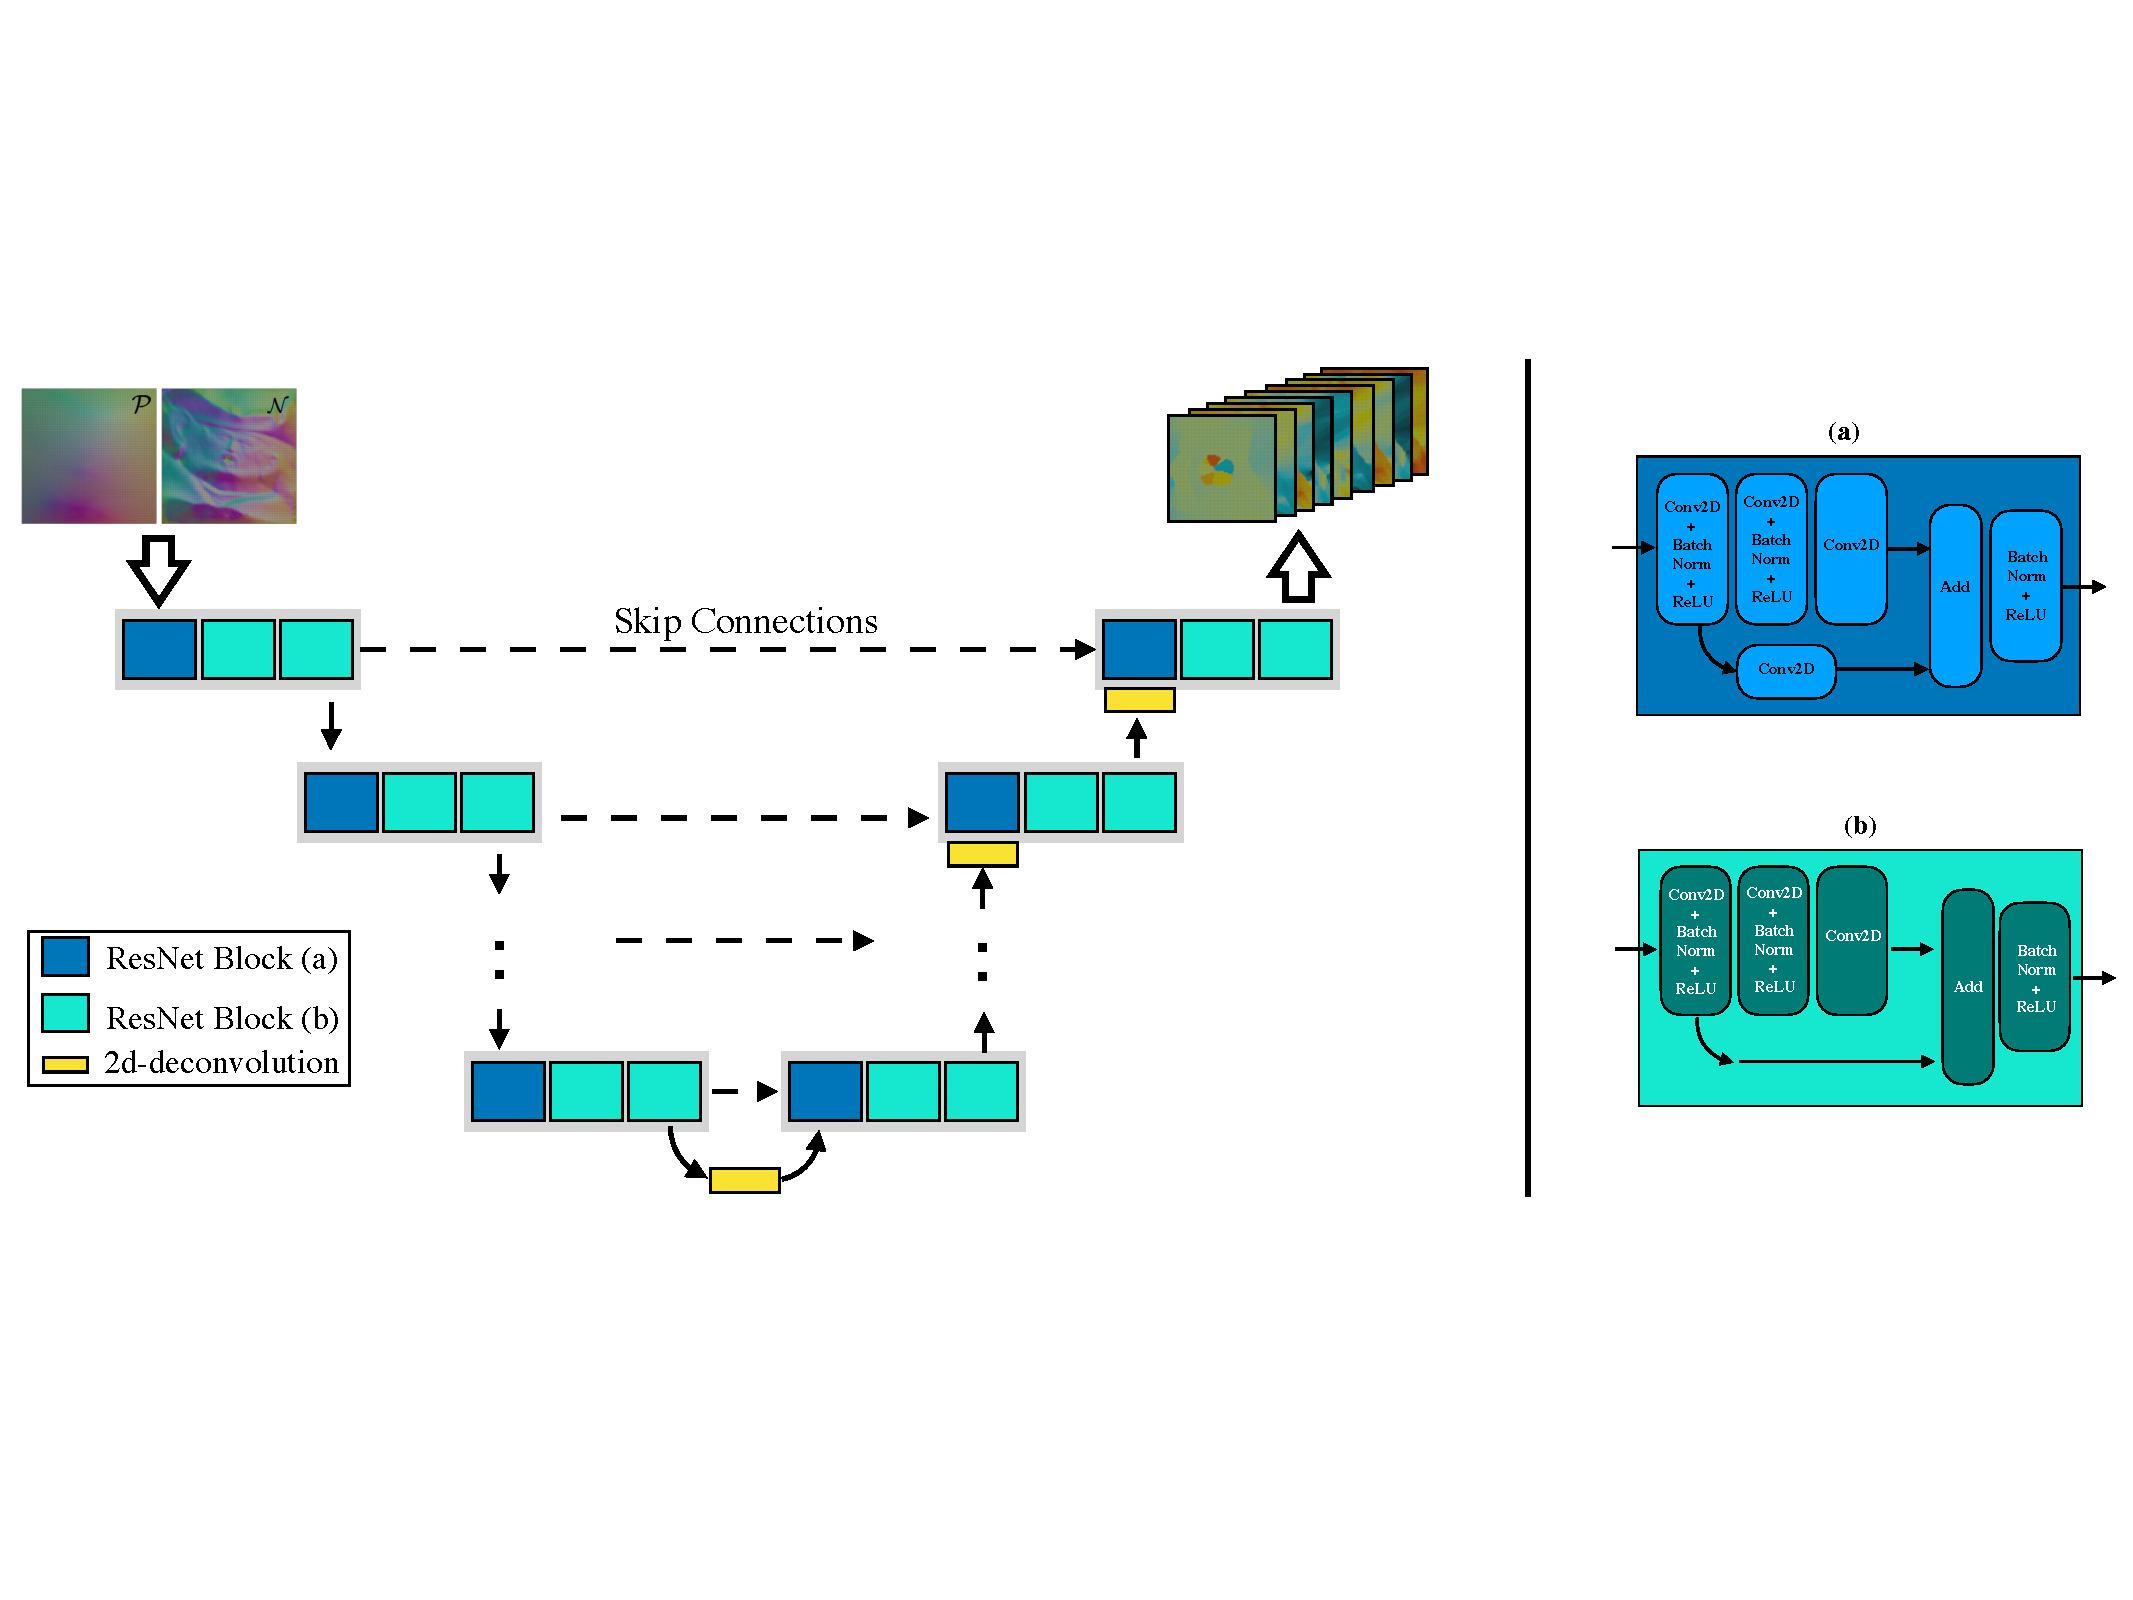
\includegraphics[width=0.7\paperwidth]{Figures/Network_topology.pdf}
     \caption{\textit{Left:} Illustration of the configuration of our U-shaped network. \textit{Right:} Shows the two kind of operations performed within our ResNet blocks.}
     \label{Fig: NetworkTopology}
\end{figure*}

  



%
% -------- RESULTS -------------

\section{Experiments and Analysis}  \label{Sec:Experiments}
We test our DeepPRT method against different animated objects: We animate a \textit{Pirate Head} and a \textit{Fish} object using a blendshape model and apply physically-based deformations to animate a \textit{Cloth} object.
The geometry image mesh resolution of the objects is $256 \times 256$. However, for the Fish object we increase the resolution to $512 \times 512$ to avoid reconstruction artifacts such as under-sampling and the limitation of harmonic mapping to recover sharp features (figure \ref{Fig: Fish Reconstruction})
% FIGURE (Fish Resampling)
\begin{figure}[H]
  \centering
    \includegraphics[width=1.0\textwidth]{Figures/fish}
     \caption{Fish reconstructions after regular sampling of squared harmonic map. \textit{Top:} Sampled by a $256 \times 256$ grid, shows detail loss and distortions. \textit{Bottom:} Higher sampling $512 \times 512$ needed to preserve detail and minimize artifacts.}
     \label{Fig: Fish Reconstruction}
\end{figure}~
These distortions arise due to the uniform remeshing, while using a sub-optimal choice of 2D surface parametrization (Harmonic Map), leading to poorly sampled surface areas in regions of higher curvatures. While sufficient for our experiments, a more suited parametrization, that minimizes distortion after resampling, is the \textit{geometric-stretch} parametrization \cite{gu2002geometry}. 
%-------------------------------------------------------------------------
%%%%% TABLE %%%%%%%%%%%
\begin{table}[h]
\begin{tabular}{|l|l|l|l|l|}
\hline
\textbf{}            & \textbf{Accuracy} & \textbf{Train-Loss} & \textbf{Val-Loss} & \multicolumn{1}{c|}{\textbf{SSIM}} \\ \hline
\textbf{Pirate} & 0.9817            & 0.000397            & 0.000399                 & 0.99386                      \\ \hline
\textbf{Fish}        & 0.9729            & 0.002104            & 0.002200                      &  0.92451                   \\ \hline
\textbf{Cloth}       & 0.9818            & 0.000078            & 0.000098                 & 0.98840                      \\ \hline
\end{tabular}
\caption{Network accuracy and SSIM are computed on training plus validation data, first and last columns respectively. Third and fourth columns show the training and validation losses of the network.} 
\label{Table: NN_Accuracy}
\end{table}

\subsection*{Quality and Memory Savings} \label{Sec: memory_savings}
For each of the test conditions, our train- and validation sets together comprise 500 distinct object deformations. 
Within that deformation set, our U-Net model is able to achieve accuracies up to 98\% (table \ref{Table: NN_Accuracy}). Moreover, the resulting rendered appearances are close to indistinguishable from the ground truth. We further quantify the quality of the results using the perceptual metric SSIM visualization (figures \ref{Fig: glossy_pirate} and \ref{Fig: DPRT_Quality}).  Based on this result, we imply that our trained network is able to faithfully approximate self-shadowing effects of 500 distinct shapes \textbf{at the very least}. Contrarily to classic PRT, which involves storing the transfer coefficients of each vertex for every single shape in the set, whilst our method only requires the storage of the network parameters. Such classic PRT data could be 10GB for a 10 second animation sequence. The weights of the neural network we produce on the other hand is only 143MB and as a fixed sized, independent of the length animation, is more uniform for practical storage allocation usage. We are able to have close results both visually and numerically to ground truth shading with our experiments. Across the metrics errors visualizations, we observe higher error regions that coincide with originating sharp features of the test objects, such that primarily follows from a limitation of harmonic maps to retain these geometric events, which may be further addressed by alternative geometry image mapping approaches.

For our particular network of approx. $11.8$ million parameters,  the example objects with $256 \times 256$ and $512 \times 512$ number of vertices, and a choice of $16$ transfer coefficients per vertex, this implies a compression ratio $r = (\text{\# PRT parameters})/(\text{\# network parameters})$ of: 
\begin{align*}
r_{diffuse} = 
\begin{cases}
\textbf{44.47 : 1} , & \mbox{for } 256^2 \mbox{ \#vertices} \\
\textbf{177.86 : 1} & \mbox{for } 512^2 \mbox{ \#vertices}
\end{cases}
\\
r_{glossy} = 
\begin{cases}
\textbf{133.41 : 1} , & \mbox{for } 256^2 \mbox{ \#vertices} \\
\textbf{533.56 : 1} & \mbox{for } 512^2 \mbox{ \#vertices}
\end{cases}
\end{align*}
for diffuse and glossy surfaces respectively. These numbers grow linearly with an increasing number of coefficients, deformations or number of vertices. 
\begin{figure}[H]
  \centering
    \includegraphics[width=0.75\textwidth]{Figures/glossy_pirate.pdf}
     \caption{Prediction of a test sample (unseen while training) for a diffuse (top) and glossy (bottom) surface. }
     \label{Fig: glossy_pirate}
\end{figure}
The measures shown above express the compression ratio taking into account solely the training and validation sets. Nevertheless, our network shows good generalization properties, also enabling accurate and qualitatively precise appearance predictions of deformations outside the training set. Hence, taking this into account the compression ratio grows significantly with potential to cover the full range of natural/possible motions for a given object within the fixed network footprint.

As mentioned above, deep neural networks can generally be further optimized, hence making DeepPRT even more efficient memory, speed and energy-wise \cite{Survey_NN_Compression}. 
%%%%%%%%%%%%%%%%%%%%%%%%%%%%%
% Comparisson 
%%%%%%%%%%%%%%%%%%%%%%%%%%%%%
\subsection*{Generality of DeepPRT and Comparison}
\subsubsection*{Generalization Capability:}
We validate the generalization capabilities of our model by standard machine learning procedures. We base our parameter tuning on minimizing the validation loss and later analyze prediction quality using a test set.

\begin{figure}[ht!]
  \centering
    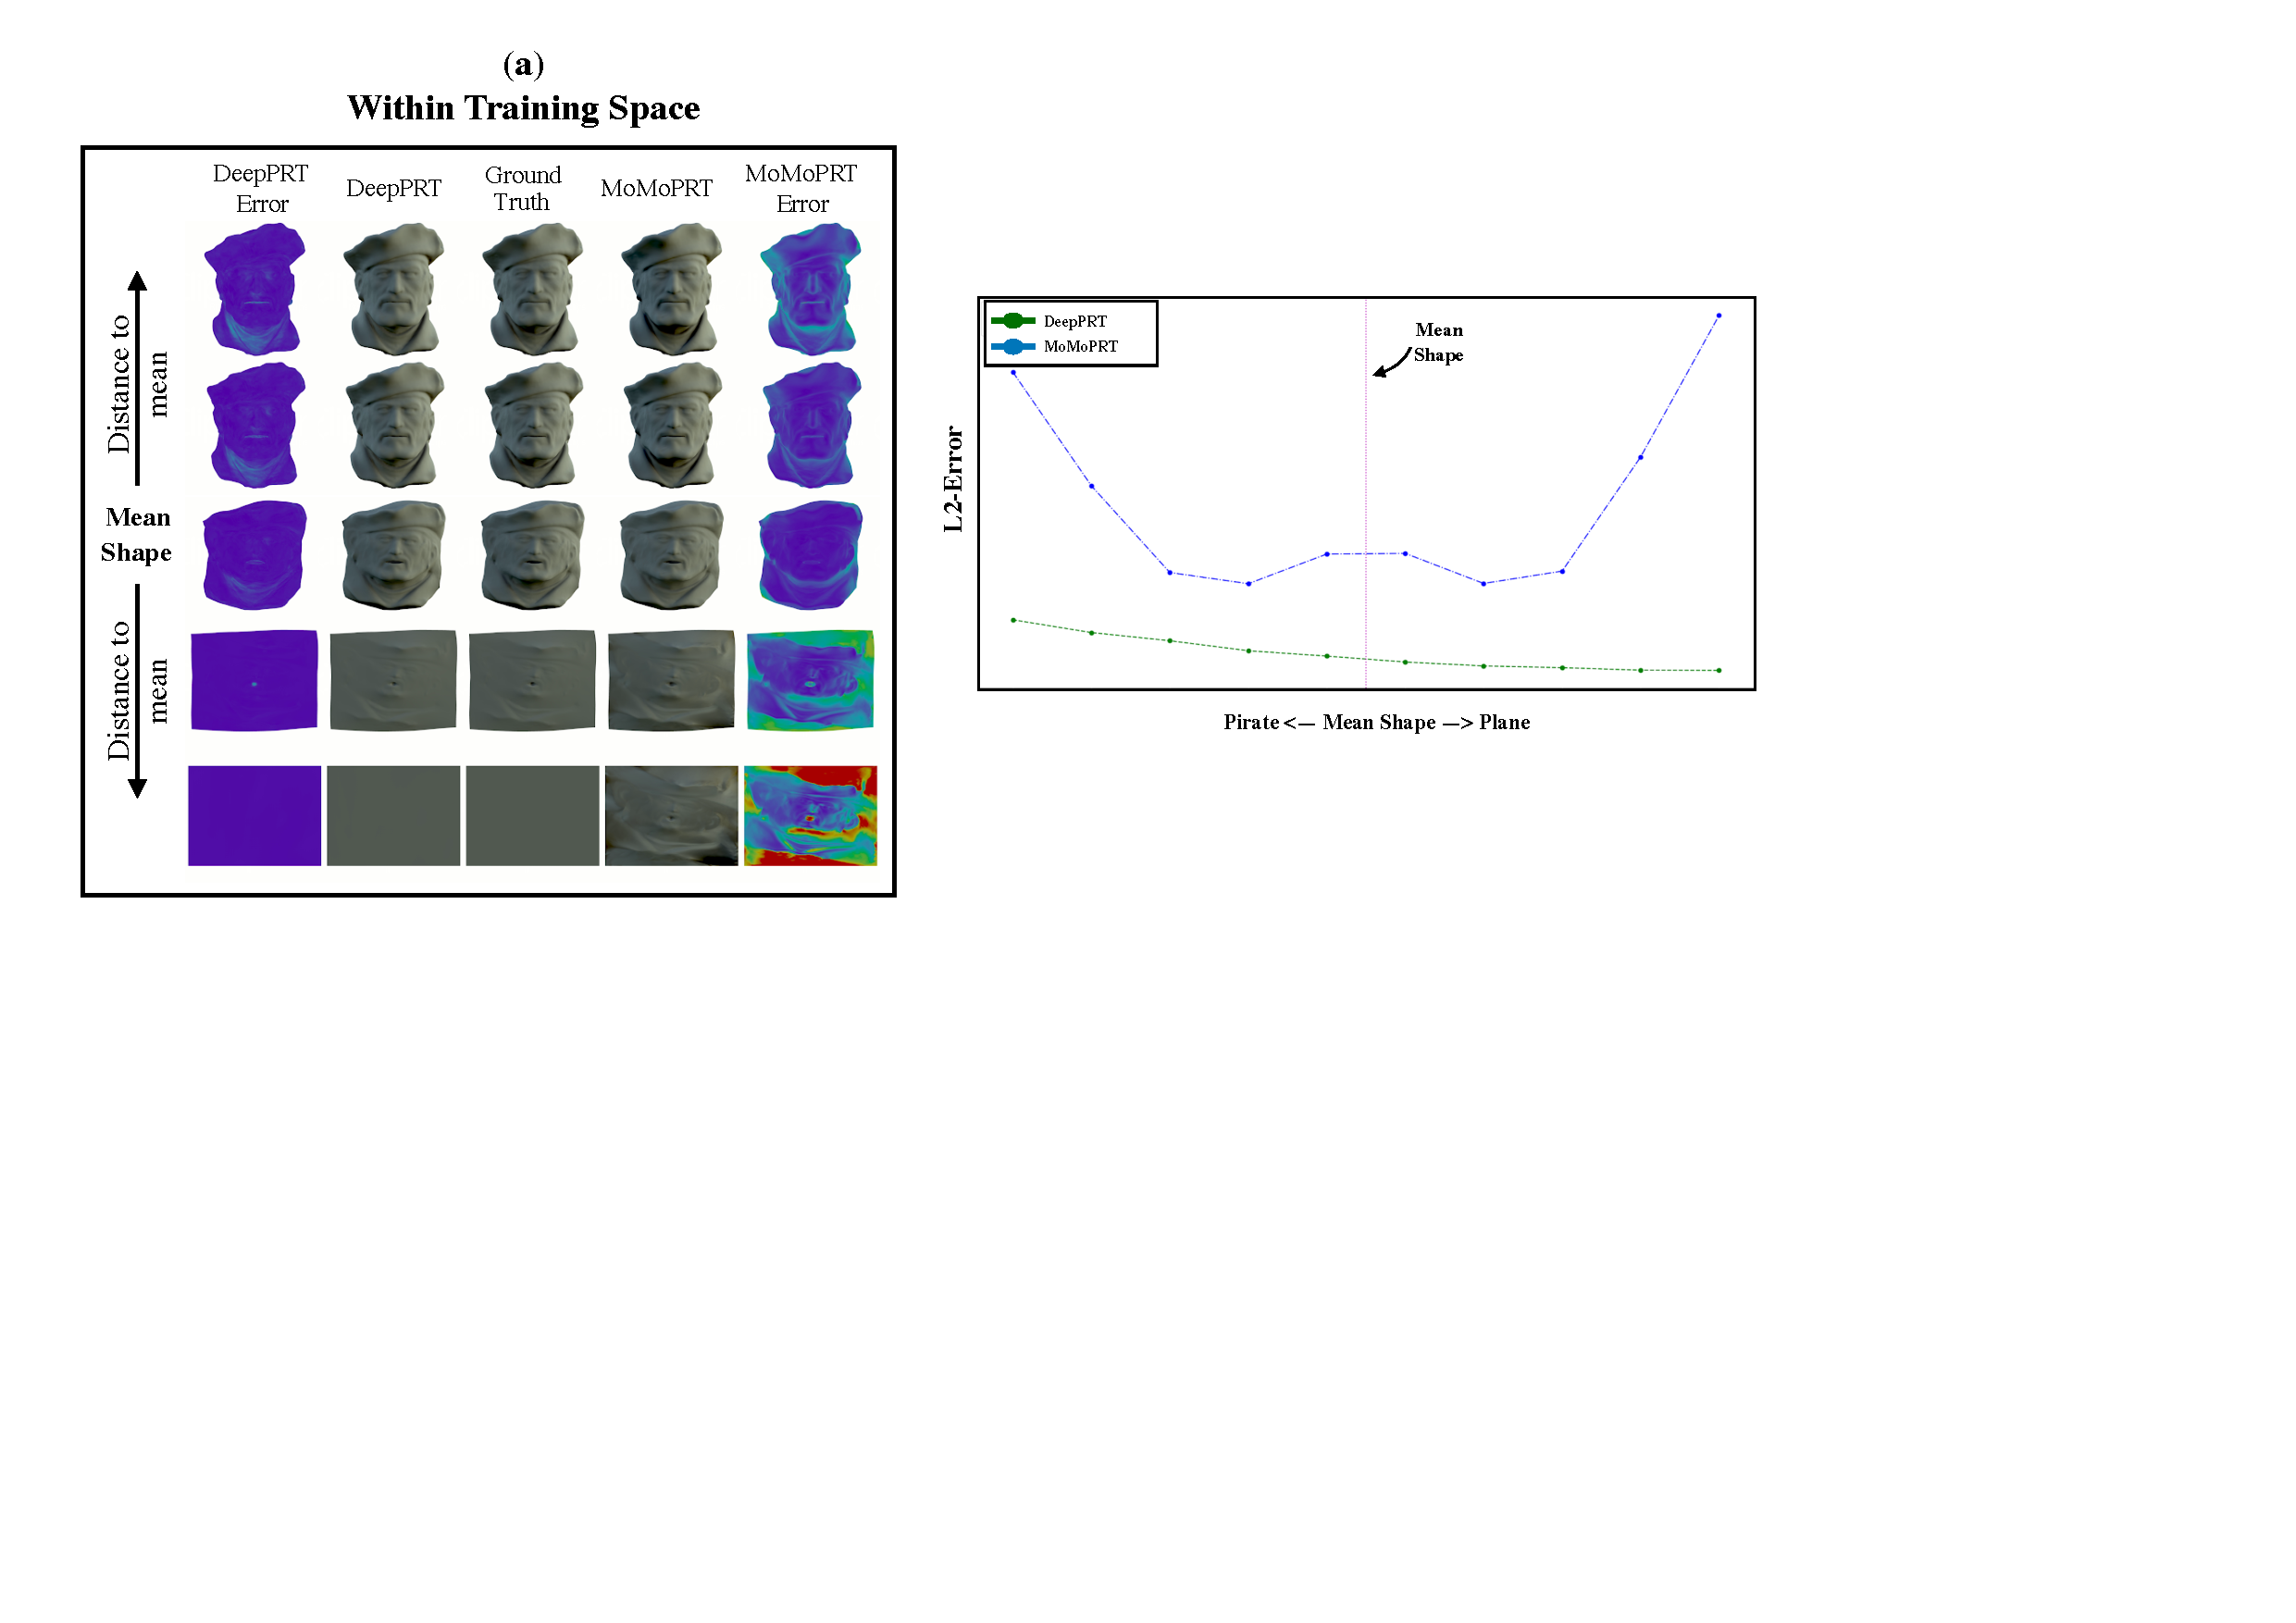
\includegraphics[width=1.0\textwidth]{Figures/DPRT_vs_MoMoPRT_aPACM.pdf}
    \includegraphics[width=1.0\textwidth]{Figures/DPRT_vs_MoMoPRT_bPACM.pdf}
     \caption{DeepPRT (ours) vs. MoMoPRT, (a) within training space and (b) moving away from the training space. \textit{ Left:} Appearance and vertex-wise $L_2$-RGB distance between ground truth and predictions.\textit{ Right:} Plot of the mean $L_2$-RGB distance for each predicted shape. DeepPRT error is lower overall and close to constant, while MoMoPRT gets worse with increasing distance to mean shape.}
     \label{Fig:DPRT vs MoMoPRT}
\end{figure}

\subsubsection*{Comparison with MoMoPRT:}
Furthermore, we compare our method with \emph{MoMoPRT} \cite{MoMoPRT} and show that DeepPRT it is more accurate and can handle more general deformations. 
Here, Schneider et al \shortcite{MoMoPRT} proposed a linear model $f_{lin}$ to predict transfer coefficients from shape parameters of a \textit{morphable model}.

Clearly, MoMoPRT is limited to shape deformations that are contained within the space described by a linear-shape-model $S_{lin}$. Moreover, although a linear model may be enough to approximate self-shadowing effects of shapes that are close to the mean shape of the data distribution of the training set, the model lacks complexity to accurately approximate data samples existing farther away from the mean shape (under-fitting).  

On the other hand, our more complex non-linear model ($f_{CNN}$) is able to capture the relationships between the dataset's features (shape) and the target variable (transfer coefficients), enabling accurate approximations for a much larger deformation domain.

For demonstration purposes, we generate a new training set consisting of $500$ shapes resulting from linear combinations between visually more dissimilar basis shapes\footnote{More distinguishable between each other, than between each face expressions used in \cite{MoMo}.}: 1) the \textit{Pirate Head } on one side, and 2)  a simple \textit{Plane} on the other. 
\begin{align*}
S_{lin} = \alpha ~ S_{pirate} + (1 - \alpha)~S_{plane}
\end{align*}
We train both models, $f_{CNN}$ and $f_{lin}$, and compute their predictions for a series of test-shapes that are evenly distributed. Figure \ref{Fig:DPRT vs MoMoPRT}a shows that the prediction accuracy of our $f_{CNN}$ model is higher and remains almost constant over the entire domain; on the contrary, the prediction accuracy of the linear model $f_{lin}$ drops significantly moving away from the mean shape (the \textit{Pirate/Plane} hybrid), as expected. 


Last but not least, we demonstrate that our model approximates data that is contained in a much larger domain than the one spanned by a linear-shape-model $S_{lin}$. The models, $f_{CNN}$ and $f_{lin}$, are fed with a series of sample shapes, starting from the mean shape and increasingly deforming towards a pirate face expression that was excluded from the training set. 

As can be seen in figure \ref{Fig:DPRT vs MoMoPRT}b, the linear model performs poorly away from $S_{lin}$, while our network's accuracy remains constant.



%
% -------- OUTLOOK -------------
\section{Conclusion and Future Work}
We present a compact representation of PRT for deformable objects in form of a non-linear model, namely a Convolutional Neural Network (CNN) that predicts the \textit{Transfer Function} for a given shape query. The model is able to capture the features of the data and generate good approximations for a wide spectrum of deformations.  As a result, our proposed CNN is able to make accurate approximations generating appearances that are visually undistinguishable from the ground truth. Moreover, our method shows much higher generalisation properties than previous approaches allowing deformations from a much larger and less constrained deformation space.\\
\\
The particular choice of our basis functions (\textit{Spherical Harmonics}), currently restricts our method to low-frequency lightings. However, an extension to all-frequencies is straught forward and can be made by fitting the model to an alternative representation of $T$, such as non-linear Wavelets \cite{AllFrequencyPRT}.\\
The most significant restrictions of our method reside within the natural flaws of \textit{Geometry Images}. Currently, our algorithm can only operate on surfaces containing one boundary and performs well for modest curvature variations. In future, alternative surface representations could be explored to overcome this restrictions.
\begin{itemize}
\item Harmonic map -> stretch min. map
\item Different NN
\item Optimisation of NN
\end{itemize}

%
% -------- REFERENCES -------------
\bibliographystyle{ACM-Reference-Format}
\bibliography{6_ref}
%
%
\end{document}